\section{Resoconto delle attività di verifica}
In questa sezione vengono descritti ed analizzati gli esiti delle attività di verifica nei vari periodi del progetto attraverso le metriche indicate precedentemente e applicate su tutti i documenti destinati alla consegna e sul prodotto da sviluppare.

\subsection{Revisione dei Requisiti}

\subsubsection{Analisi statica dei documenti}
I membri del gruppo \Gruppo{} hanno analizzato i documenti mediante la tecnica di walkthrough che ha portato all'individuazione di 
alcuni errori ortografici e grammaticali, grazie anche agli strumenti di controllo ortografico integrati negli editor per la produzione
della documentazione che il gruppo ha deciso di utilizzare.

\subsubsection{Esiti verifiche automatizzate}
Attualmente, l'unico valore che può essere calcolato per \glo{verificare} se la garanzia di qualità che il gruppo ritiene fornire è
soddisfatta, è data dall'Indice di Gulpease (MPC6).
Nella seguente tabella sono riportati i risultati degli indici di Gulpease ottenuti dai documenti per la fase di Analisi.
In seguito vi è un grafico che riporterà l'andamento degli indici di Gulpease per ogni documento.

\paragraph{MPC6 - Indice di Gulpease}
\subparagraph*{Legenda}
\begin{itemize}
	\item \textbf{Documento}: Nome del documento;
	\item \textbf{RR}: Fase di Revisione dei Requisiti;
	\item \textbf{Colore rosso}: Indica che il valore ottenuto non è accettabile;
	\item \textbf{Colore giallo}: Indica che il valore ottenuto è accettabile;
	\item \textbf{Colore verde}: Indica che il valore ottenuto è ottimo. 
\end{itemize}

\rowcolors{2}{grigetto}{white}
\renewcommand{\arraystretch}{1.5}
\begin{longtable}{C{4cm} C{1cm} C{1cm} C{1cm}}% C{1cm}}
\caption{Elenco degli indici di Gulpease }\\
\rowcolor{darkblue}
\textcolor{white}{\textbf{Documento}} & \textcolor{white}{\textbf{RR}} \\ % & \textcolor{white}{\textbf{RP}} \\
\hline
\endhead
\AdR & \textcolor{verde}{\textbf{95}} \\% & \textcolor{verde}{\textbf{83}} \\
\PdP & \textcolor{verde}{\textbf{100}} \\ % & \textcolor{verde}{\textbf{100}} \\
\PdQ & \textcolor{verde}{\textbf{100}}\\% & \textcolor{verde}{\textbf{92}} \\

\NdP & \textcolor{giallo}{\textbf{75}}\\% & \textcolor{giallo}{\textbf{76}} \\
\SdF & \textcolor{verde}{\textbf{94}} \\% & \textcolor{verde}{\textbf{94}} \\

\Glossario & \textcolor{giallo}{\textbf{67}}\\ % & \textcolor{giallo}{\textbf{75}} \\

Media verbali interni & \textcolor{verde}{\textbf{92}}\\ % & \textcolor{verde}{\textbf{87}} \\
Media verbali esterni & \textcolor{giallo}{\textbf{65}}\\ % & \textcolor{giallo}{\textbf{70}} \\

\end{longtable}
\newpage
\pgfplotsset{width=17cm, height=10cm}
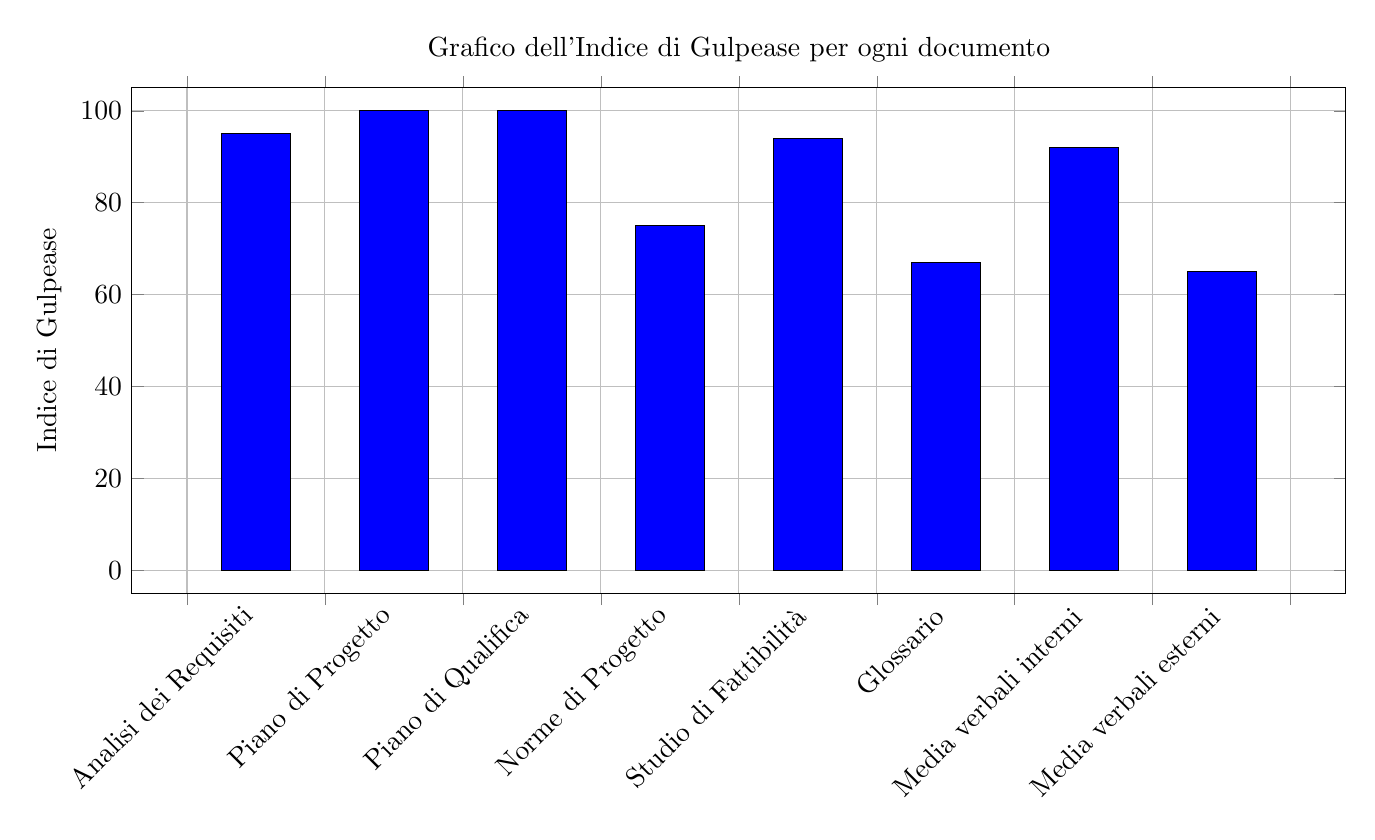
\begin{tikzpicture}

\begin{axis}[
title=Grafico dell'Indice di Gulpease per ogni documento,
x tick label style={
/pgf/number format/1000 sep=},
ylabel=Indice di Gulpease,
enlargelimits=0.05,
legend style={at={(0.5,-0.4)},
anchor=north,legend columns=-1},
ybar interval=0.5,
symbolic x coords={Analisi dei Requisiti, Piano di Progetto, Piano di Qualifica, Norme di Progetto, Studio di Fattibilità, Glossario,
Media verbali interni, Media verbali esterni, tmp},%lasciare tmp come ultima colonna per poter visualizzare tutte le colonne tranne tmp
x tick label style={rotate=45,anchor=east},
grid=major,
xtick=data
]
\addplot[fill=blue] coordinates
{(Analisi dei Requisiti, 95) (Piano di Progetto, 100) (Piano di Qualifica, 100) 
(Norme di Progetto, 75) (Studio di Fattibilità, 94) (Glossario, 67)
(Media verbali interni, 92) (Media verbali esterni, 65) (tmp, 0)};

\end{axis}
\end{tikzpicture}
\newpage

\subsection{Revisione di progettazione}
\subsubsection{Analisi statica dei documenti}
In questa fase i membri del gruppo \Gruppo{} hanno analizzato i documenti mediante la tecnica dell'\glo{inspection}, abbandonando la tecnica di \glo{walkthrough} dato che il gruppo ha acquisito abbastanza esperienza, riducendo così i costi di verifica. In questo periodo sono stati corretti gli errori riscontrati e aggiornati i vari documenti portandoli a una nuova versione di rilascio.

\subsubsection{Analisi statica del codice}
In questo periodo il gruppo è stato molto impegnato nello sviluppo del \glo{Proof of Concept}, perciò è stato necessario adottarsi di strumenti per la stesura e la verifica statica del codice. 

\subsubsection{Esiti verifiche automatizzate}
Di seguito verranno mostrati gli esiti delle metriche che si sono riuscite a calcolare. Purtroppo, non è stato possibile calcolare le metriche \textbf{MPC7} e \textbf{MPD7}. \\ Dopo la visione degli esiti ci sarà una sezione dedicata all'analisi dei risultati.

\paragraph{MPC1 - Percentuale requisiti obbligatori soddisfatti} 

\pgfplotsset{width=17cm, height=8cm}
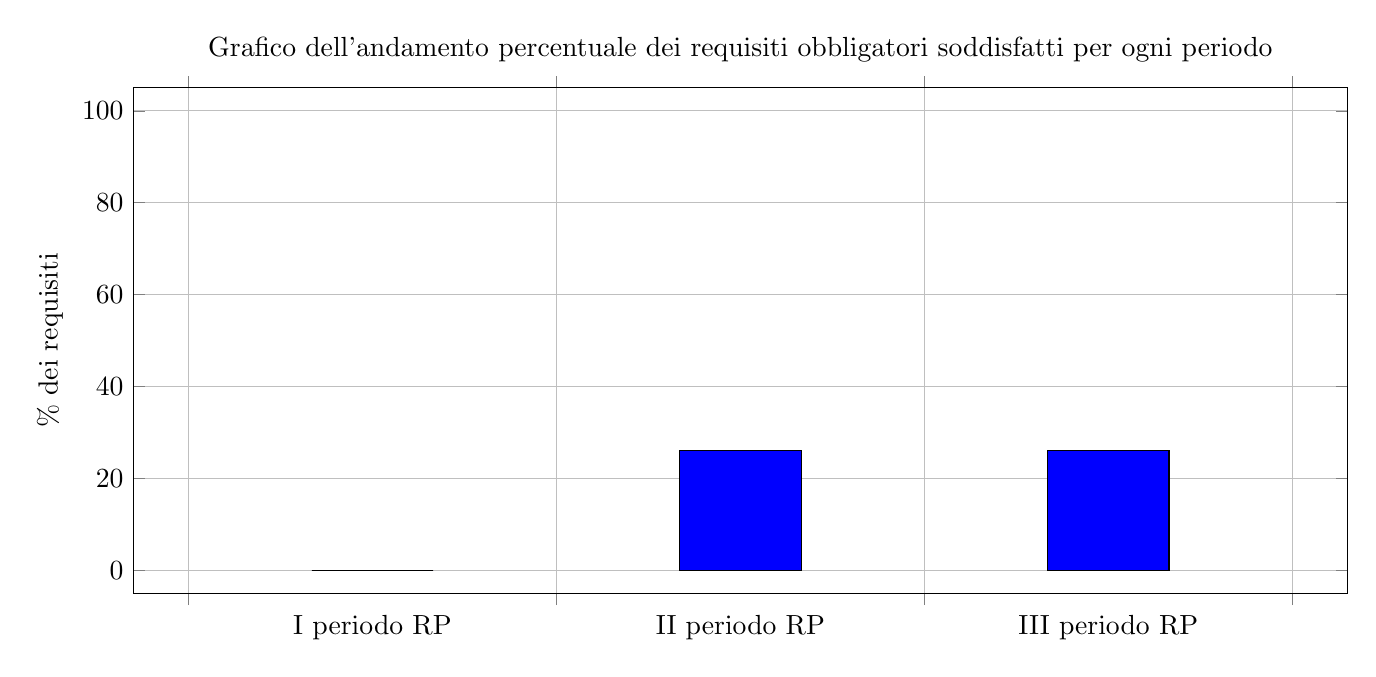
\begin{tikzpicture}

\begin{axis}[
title=Grafico dell'andamento percentuale dei requisiti obbligatori soddisfatti per ogni periodo,
x tick label style={
	/pgf/number format/1000 sep=},
ylabel=\% dei requisiti,
enlargelimits=0.05,
legend style={at={(0.5,-0.4)},
	anchor=north,legend columns=-1},
ybar interval=0.33,
symbolic x coords={I periodo RP, II periodo RP, III periodo RP, tmp},%lasciare tmp come ultima colonna per poter visualizzare tutte le colonne tranne tmp
grid=major,
xtick=data
]
\addplot[fill=blue] coordinates
{(I periodo RP, 0) (II periodo RP, 26) (III periodo RP, 26) (tmp, 100)};

\end{axis}
\end{tikzpicture}

\paragraph{MPC2 - Incapsulamento CBO}

\pgfplotsset{width=17cm, height=8cm}
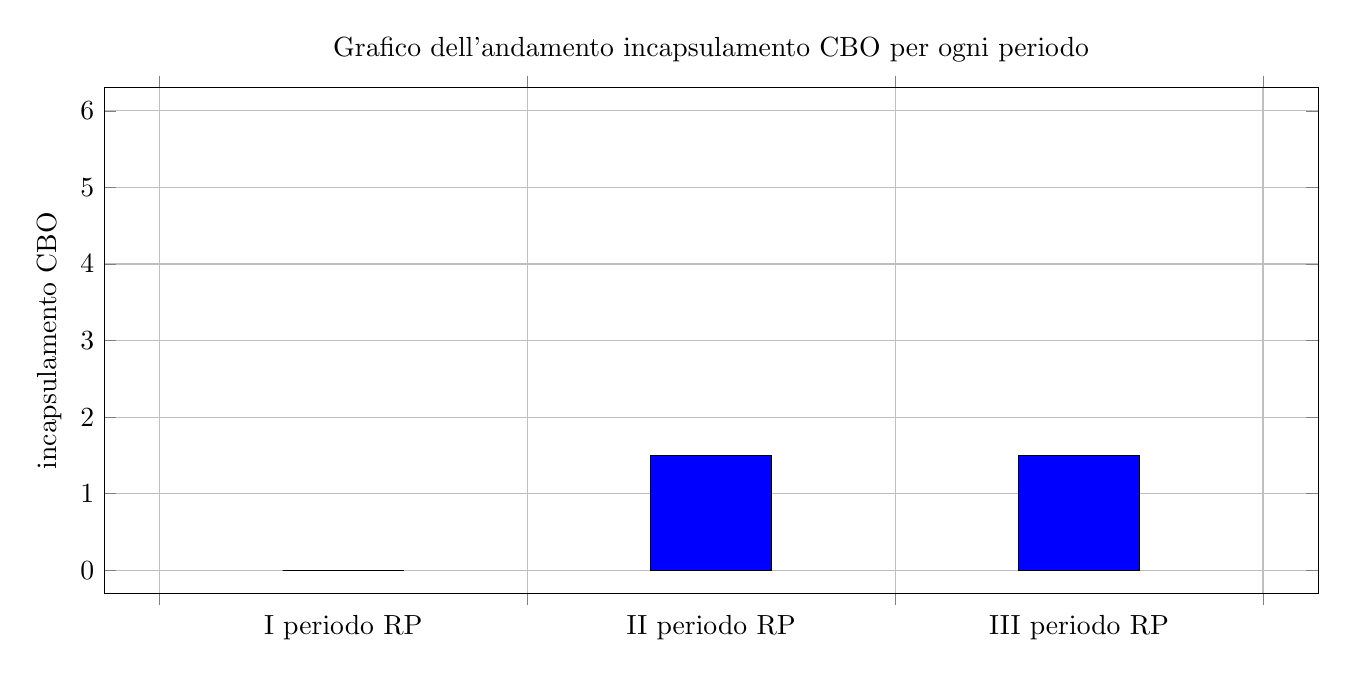
\begin{tikzpicture}

\begin{axis}[
title=Grafico dell'andamento incapsulamento CBO per ogni periodo,
x tick label style={
	/pgf/number format/1000 sep=},
ylabel=incapsulamento CBO,
enlargelimits=0.05,
legend style={at={(0.5,-0.4)},
	anchor=north,legend columns=-1},
ybar interval=0.33,
symbolic x coords={I periodo RP, II periodo RP, III periodo RP, tmp},%lasciare tmp come ultima colonna per poter visualizzare tutte le colonne tranne tmp
grid=major,
xtick=data
]
\addplot[fill=blue] coordinates
{(I periodo RP, 0) (II periodo RP, 1.5) (III periodo RP, 1.5) (tmp, 6)};
\end{axis}
\end{tikzpicture}

\paragraph{MPC3 - Livello profondità gerarchia}

\pgfplotsset{width=17cm, height=8cm}
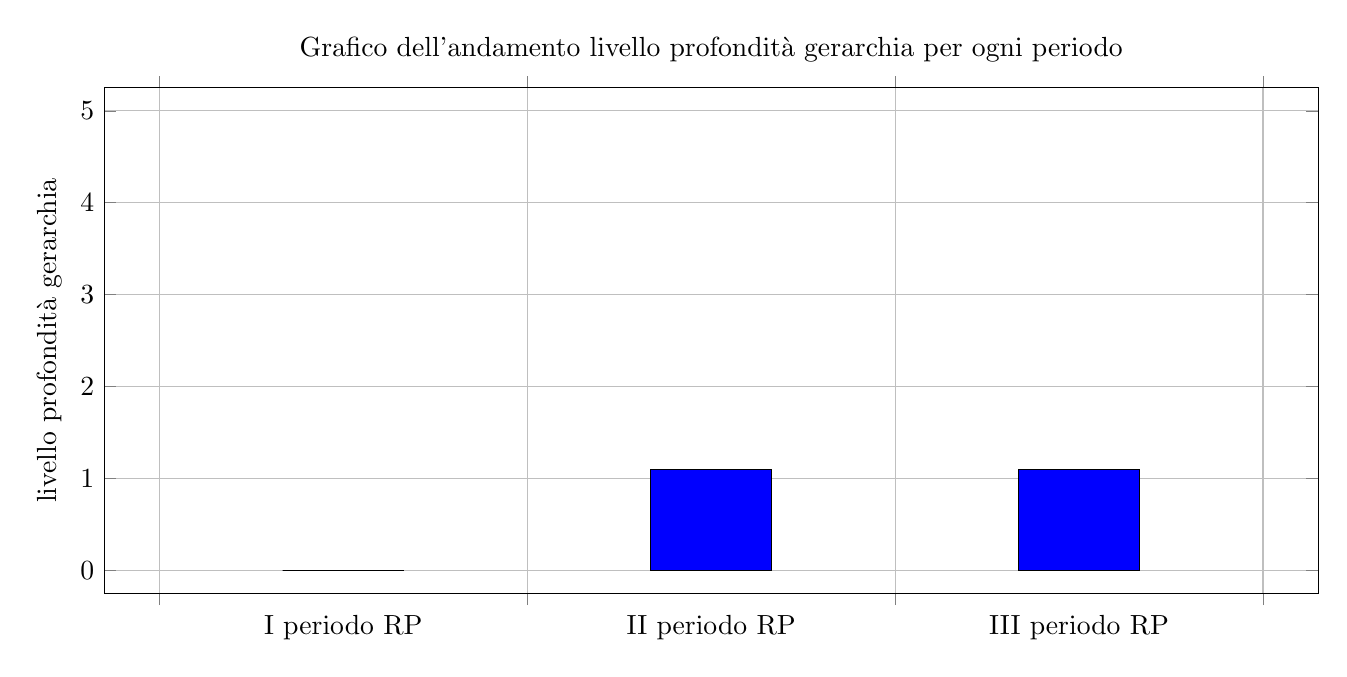
\begin{tikzpicture}

\begin{axis}[
title=Grafico dell'andamento livello profondità gerarchia per ogni periodo,
x tick label style={
	/pgf/number format/1000 sep=},
ylabel=livello profondità gerarchia,
enlargelimits=0.05,
legend style={at={(0.5,-0.4)},
	anchor=north,legend columns=-1},
ybar interval=0.33,
symbolic x coords={I periodo RP, II periodo RP, III periodo RP, tmp},%lasciare tmp come ultima colonna per poter visualizzare tutte le colonne tranne tmp
grid=major,
xtick=data
]
\addplot[fill=blue] coordinates
{(I periodo RP, 0) (II periodo RP, 1.1) (III periodo RP, 1.1) (tmp, 5)};

\end{axis}
\end{tikzpicture}

\paragraph{MPC4 - Numero di parametri per metodo}

\pgfplotsset{width=17cm, height=8cm}
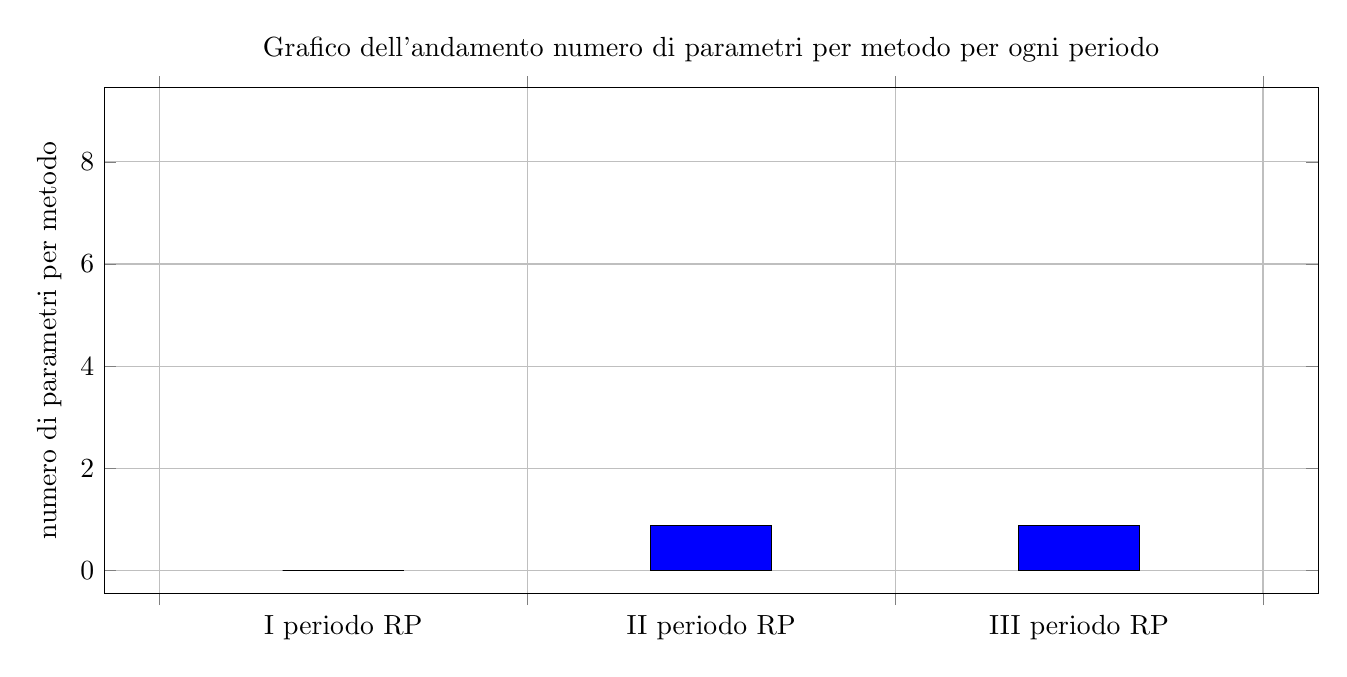
\begin{tikzpicture}

\begin{axis}[
title=Grafico dell'andamento numero di parametri per metodo per ogni periodo,
x tick label style={
	/pgf/number format/1000 sep=},
ylabel=numero di parametri per metodo,
enlargelimits=0.05,
legend style={at={(0.5,-0.4)},
	anchor=north,legend columns=-1},
ybar interval=0.33,
symbolic x coords={I periodo RP, II periodo RP, III periodo RP, tmp},%lasciare tmp come ultima colonna per poter visualizzare tutte le colonne tranne tmp
grid=major,
xtick=data
]
\addplot[fill=blue] coordinates
{(I periodo RP, 0) (II periodo RP, 0.87) (III periodo RP, 0.87) (tmp, 9)};

\end{axis}
\end{tikzpicture}

\paragraph{MPC5 - Linee di commento per linee di codice}
\pgfplotsset{width=17cm, height=8cm}
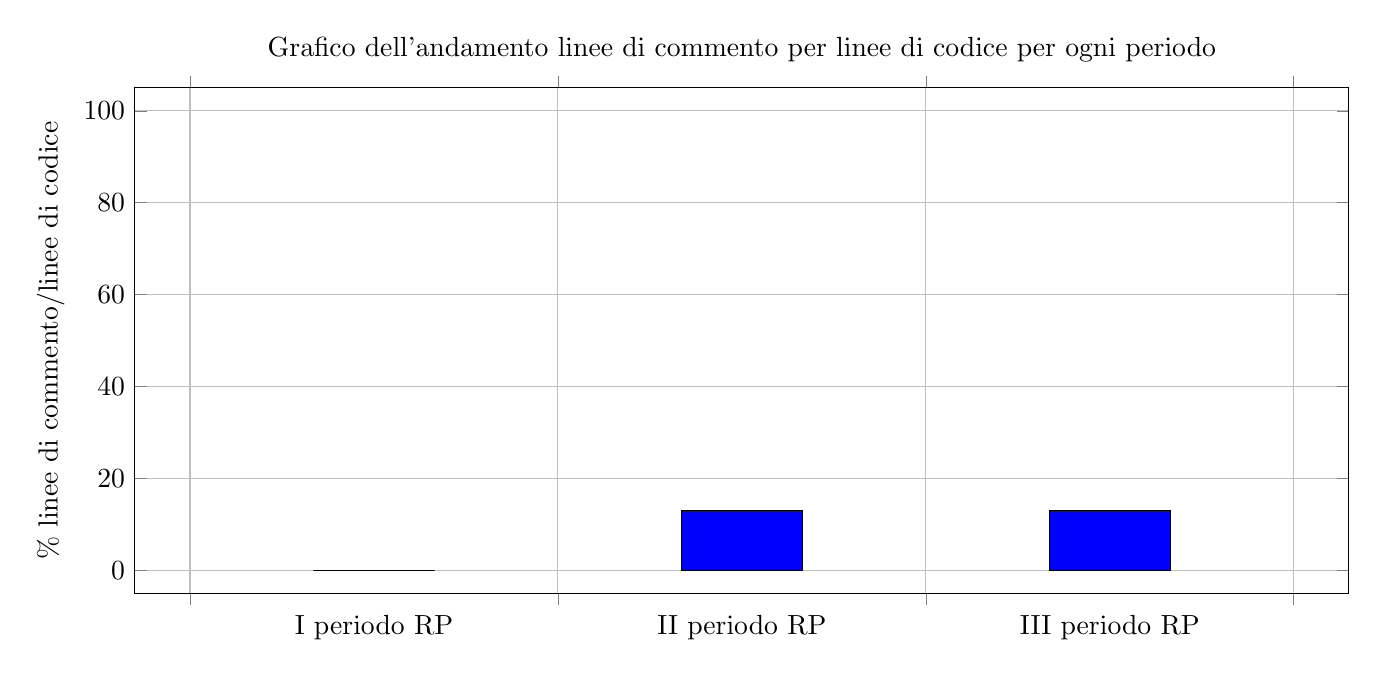
\begin{tikzpicture}

\begin{axis}[
title=Grafico dell'andamento linee di commento per linee di codice per ogni periodo,
x tick label style={
	/pgf/number format/1000 sep=},
ylabel=\% linee di commento/linee di codice,
enlargelimits=0.05,
legend style={at={(0.5,-0.4)},
	anchor=north,legend columns=-1},
ybar interval=0.33,
symbolic x coords={I periodo RP, II periodo RP, III periodo RP, tmp},%lasciare tmp come ultima colonna per poter visualizzare tutte le colonne tranne tmp
grid=major,
xtick=data
]
\addplot[fill=blue] coordinates
{(I periodo RP, 0) (II periodo RP, 13) (III periodo RP, 13) (tmp, 100)};

\end{axis}
\end{tikzpicture}
\newpage

\paragraph{MPC6 - Indice di Gulpease}
\subparagraph*{Legenda}
\begin{itemize}
	\item \textbf{Documento}: Nome del documento;
	\item \textbf{RP}: Periodo di Revisione di Progettazione;
	\item \textbf{Colore rosso}: Indica che il valore ottenuto non è accettabile;
	\item \textbf{Colore giallo}: Indica che il valore ottenuto è accettabile;
	\item \textbf{Colore verde}: Indica che il valore ottenuto è ottimo. 
\end{itemize}

\rowcolors{2}{grigetto}{white}
\renewcommand{\arraystretch}{1.5}
\begin{longtable}{C{4cm} C{2cm} C{2cm} C{2cm} C{2cm}}
	\caption{Elenco degli indici di Gulpease }\\
	\rowcolor{darkblue}
	\textcolor{white}{\textbf{Documento}} & \textcolor{white}{\textbf{I periodo RP}} &
	\textcolor{white}{\textbf{II periodo RP}} & \textcolor{white}{\textbf{III periodo RP}} \\
	\hline
	\endhead
	\AdR & \textcolor{verde}{\textbf{83}} & \textcolor{verde}{\textbf{83}} & \textcolor{verde}{\textbf{83}} \\
	\PdP & \textcolor{verde}{\textbf{100}} & \textcolor{verde}{\textbf{100}} & \textcolor{verde}{\textbf{96}} \\
	\PdQ & \textcolor{verde}{\textbf{92}} & \textcolor{verde}{\textbf{92}} & \textcolor{verde}{\textbf{90}} \\

	\NdP & \textcolor{giallo}{\textbf{76}} & \textcolor{giallo}{\textbf{76}} & \textcolor{giallo}{\textbf{77}} \\
	\SdF & \textcolor{verde}{\textbf{94}} & \textcolor{verde}{\textbf{94}} & \textcolor{verde}{\textbf{94}} \\

	\Glossario & \textcolor{giallo}{\textbf{75}} & \textcolor{giallo}{\textbf{75}} & \textcolor{giallo}{\textbf{75}} \\

	Media verbali interni & \textcolor{verde}{\textbf{87}} & \textcolor{verde}{\textbf{87}} & \textcolor{verde}{\textbf{87}} \\
	Media verbali esterni & \textcolor{giallo}{\textbf{70}} & \textcolor{giallo}{\textbf{70}}  & \textcolor{giallo}{\textbf{70}} \\
	
\end{longtable}

\pgfplotsset{width=17cm, height=9cm}
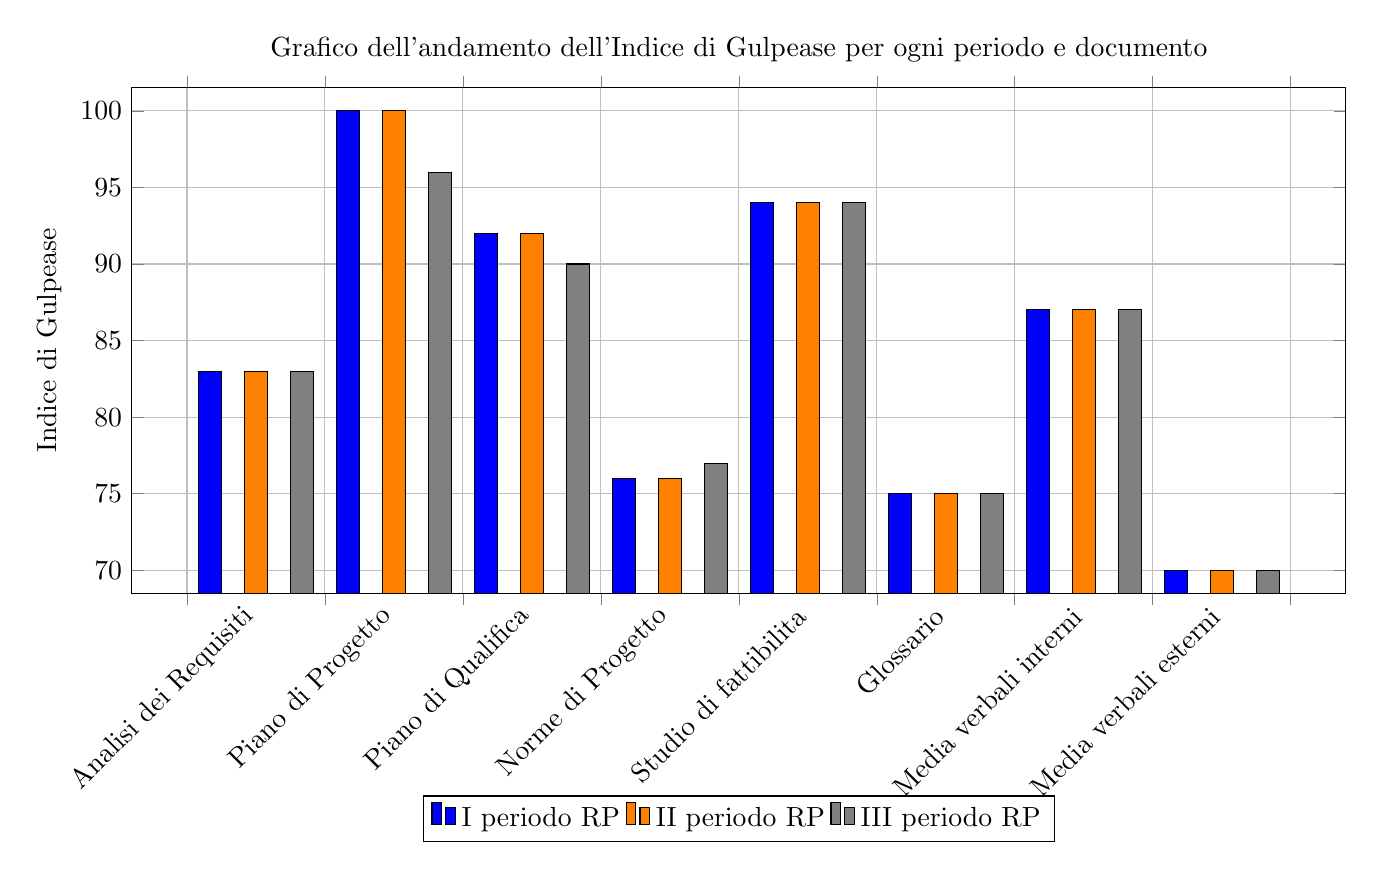
\begin{tikzpicture}

\begin{axis}[
title=Grafico dell'andamento dell'Indice di Gulpease per ogni periodo e documento,
x tick label style={
	/pgf/number format/1000 sep=},
ylabel=Indice di Gulpease,
enlargelimits=0.05,
legend style={at={(0.5,-0.4)},
	anchor=north,legend columns=-1},
ybar interval=0.5,
symbolic x coords={Analisi dei Requisiti, Piano di Progetto, Piano di Qualifica, Norme di Progetto, Studio di fattibilita, Glossario,
	Media verbali interni, Media verbali esterni, tmp},%lasciare tmp come ultima colonna per poter visualizzare tutte le colonne tranne tmp
x tick label style={rotate=45,anchor=east},
grid=major,
xtick=data
]
\addplot[fill=blue] coordinates
{(Analisi dei Requisiti, 83) (Piano di Progetto, 100) (Piano di Qualifica, 92) 
	(Norme di Progetto, 76) (Studio di fattibilita, 94) (Glossario, 75)
	(Media verbali interni, 87) (Media verbali esterni, 70) (tmp, 100)};

\addplot [fill=orange] coordinates
{(Analisi dei Requisiti, 83) (Piano di Progetto, 100) (Piano di Qualifica, 92) 
	(Norme di Progetto, 76) (Studio di fattibilita, 94) (Glossario, 75)
	(Media verbali interni, 87) (Media verbali esterni, 70) (tmp, 100)};

\addplot [fill=gray] coordinates
{(Analisi dei Requisiti, 83) (Piano di Progetto, 96) (Piano di Qualifica, 90) 
	(Norme di Progetto, 77) (Studio di fattibilita, 94) (Glossario, 75) 
	(Media verbali interni, 87) (Media verbali esterni, 70) (tmp, 100)};



\legend{
	I periodo RP,
	II periodo RP,
	III periodo RP
}
\end{axis}
\end{tikzpicture}

\paragraph{MPC8 - Actual Cost of Work Performed}
\pgfplotsset{width=17cm, height=8cm}
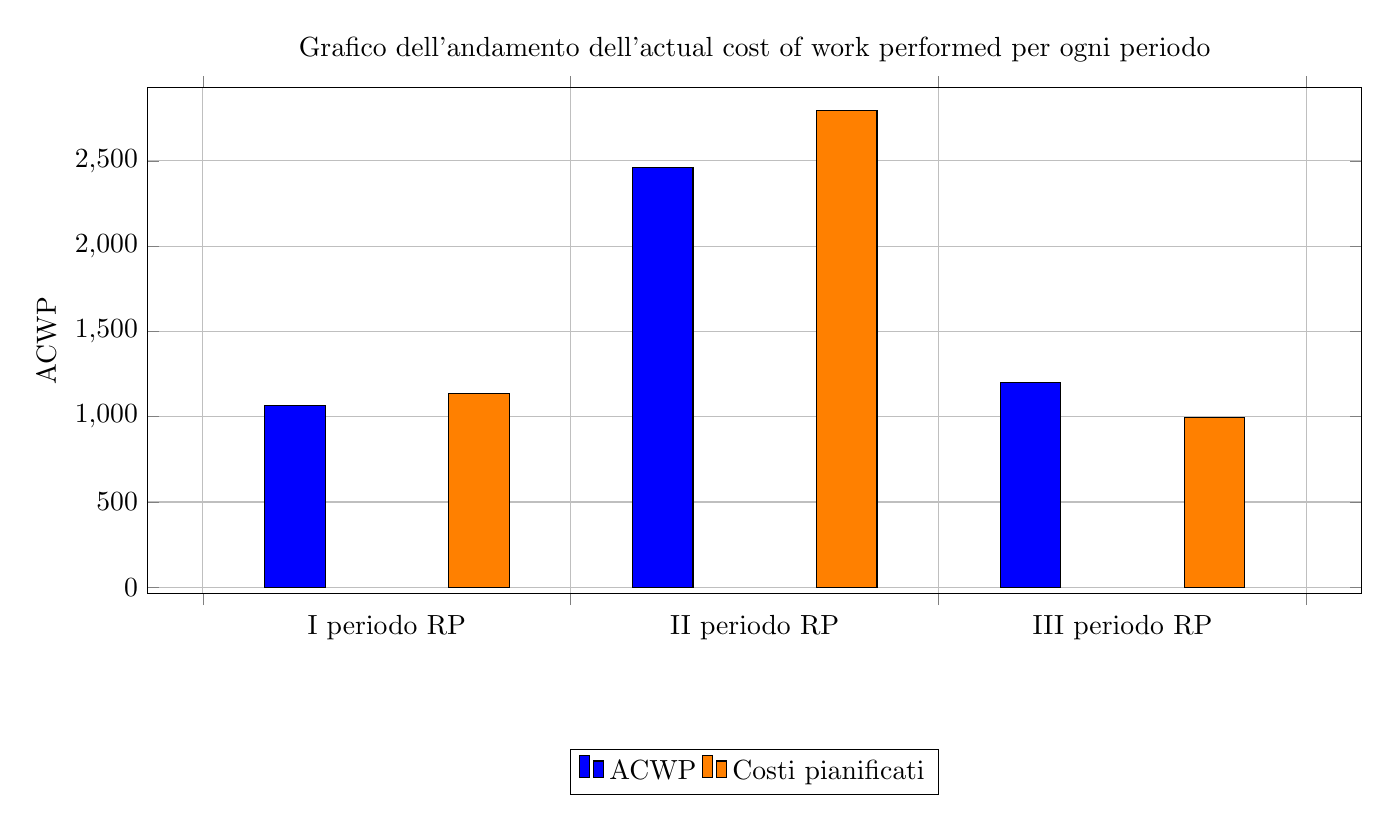
\begin{tikzpicture}

\begin{axis}[
title=Grafico dell'andamento dell'actual cost of work performed per ogni periodo,
x tick label style={
	/pgf/number format/1000 sep=},
ylabel=ACWP,
enlargelimits=0.05,
legend style={at={(0.5,-0.4)},
	anchor=north,legend columns=-1},
ybar interval=0.33,
symbolic x coords={I periodo RP, II periodo RP, III periodo RP, tmp},%lasciare tmp come ultima colonna per poter visualizzare tutte le colonne tranne tmp
grid=major,
legend style={at={(0.5,-0.4)},
	anchor=south,legend columns=-1},
xtick=data
]
\addplot[fill=blue] coordinates
{(I periodo RP, 1065) (II periodo RP, 2462) (III periodo RP, 1200) (tmp, 100)};
\addplot[fill=orange] coordinates
{(I periodo RP, 1135) (II periodo RP, 2793) (III periodo RP, 995) (tmp, 100)};

\legend{
	ACWP,
	Costi pianificati
}
\end{axis}
\end{tikzpicture}

\paragraph{MPC9 - Budgeted Cost of Work Scheduled}
\pgfplotsset{width=17cm, height=8cm}
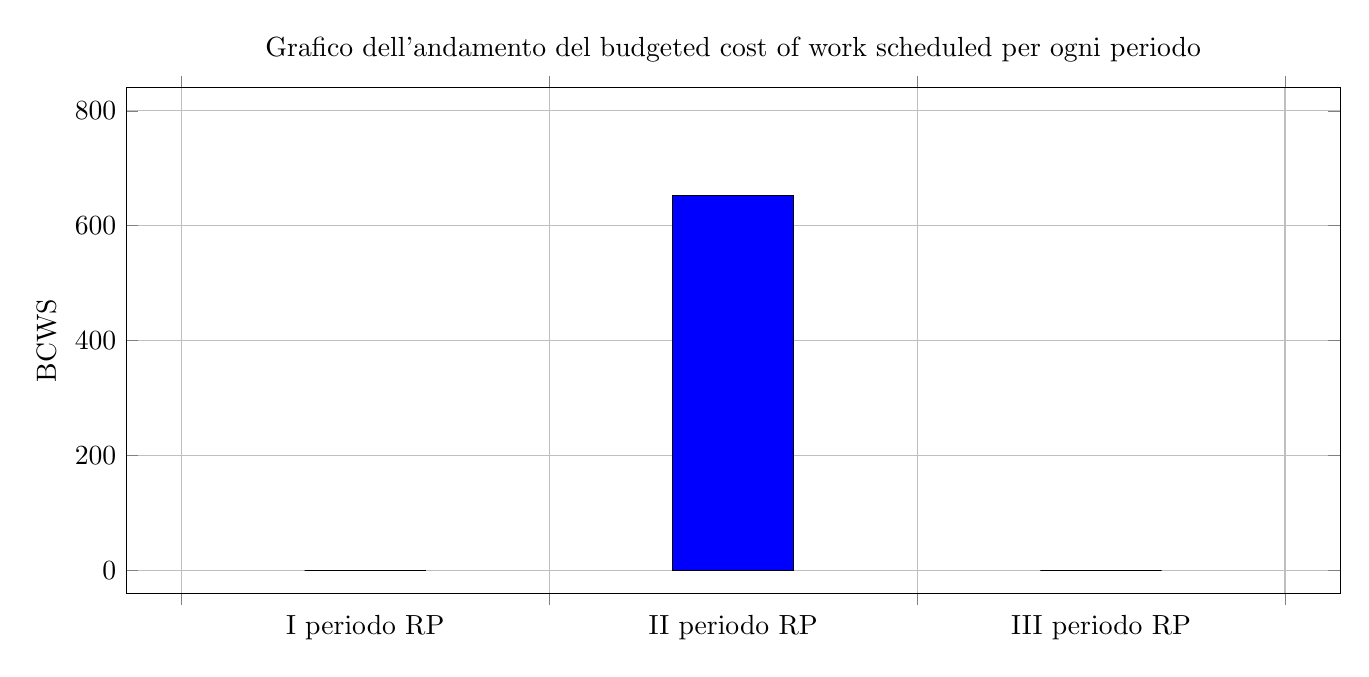
\begin{tikzpicture}

\begin{axis}[
title=Grafico dell'andamento del budgeted cost of work scheduled per ogni periodo,
x tick label style={
	/pgf/number format/1000 sep=},
ylabel=BCWS,
enlargelimits=0.05,
legend style={at={(0.5,-0.4)},
	anchor=north,legend columns=-1},
ybar interval=0.33,
symbolic x coords={I periodo RP, II periodo RP, III periodo RP, tmp},%lasciare tmp come ultima colonna per poter visualizzare tutte le colonne tranne tmp
grid=major,
xtick=data
]
\addplot[fill=blue] coordinates
{(I periodo RP, 0) (II periodo RP, 653) (III periodo RP, 0) (tmp, 800)};

\end{axis}
\end{tikzpicture}

\paragraph{MPC10 - Budgeted Cost of Work Performed}
\pgfplotsset{width=17cm, height=8cm}
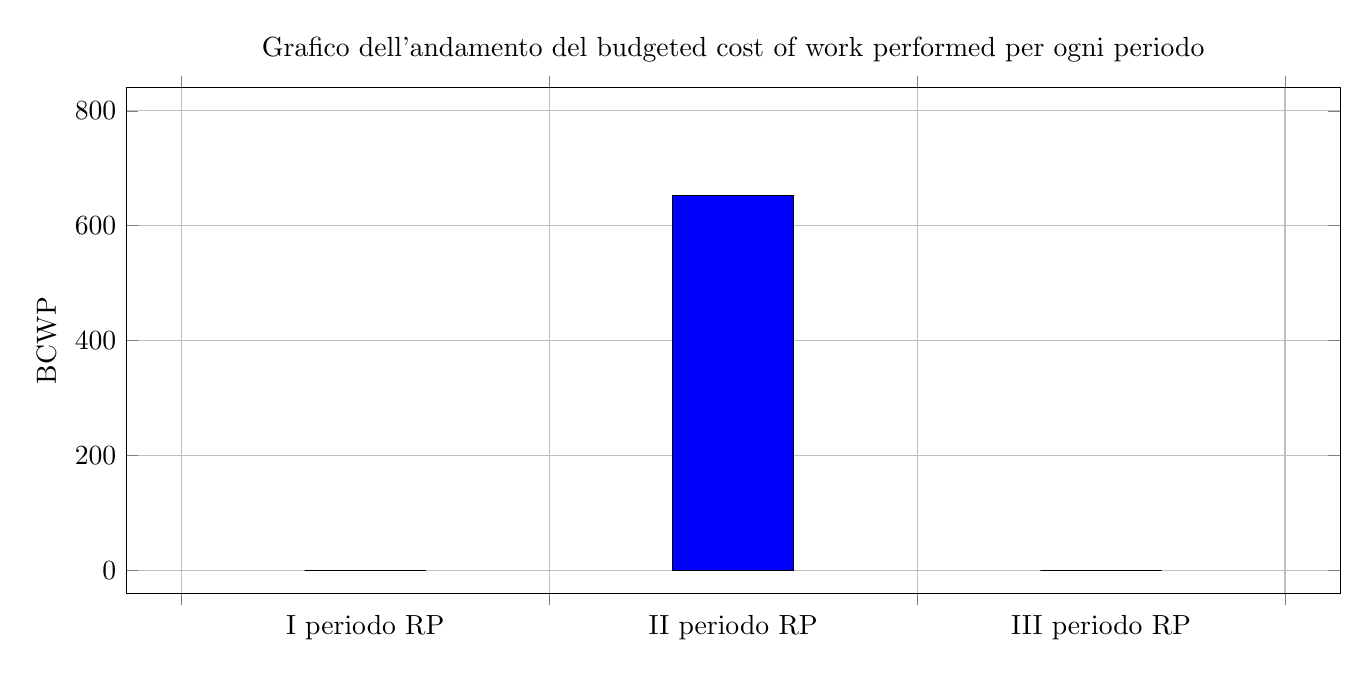
\begin{tikzpicture}

\begin{axis}[
title=Grafico dell'andamento del budgeted cost of work performed per ogni periodo,
x tick label style={
	/pgf/number format/1000 sep=},
ylabel=BCWP,
enlargelimits=0.05,
legend style={at={(0.5,-0.4)},
	anchor=north,legend columns=-1},
ybar interval=0.33,
symbolic x coords={I periodo RP, II periodo RP, III periodo RP, tmp},%lasciare tmp come ultima colonna per poter visualizzare tutte le colonne tranne tmp
grid=major,
xtick=data
]
\addplot[fill=blue] coordinates
{(I periodo RP, 0) (II periodo RP, 653) (III periodo RP, 0) (tmp, 800)};

\end{axis}
\end{tikzpicture}


\paragraph{MPC11 - Schedule Variance}
\pgfplotsset{width=17cm, height=8cm}
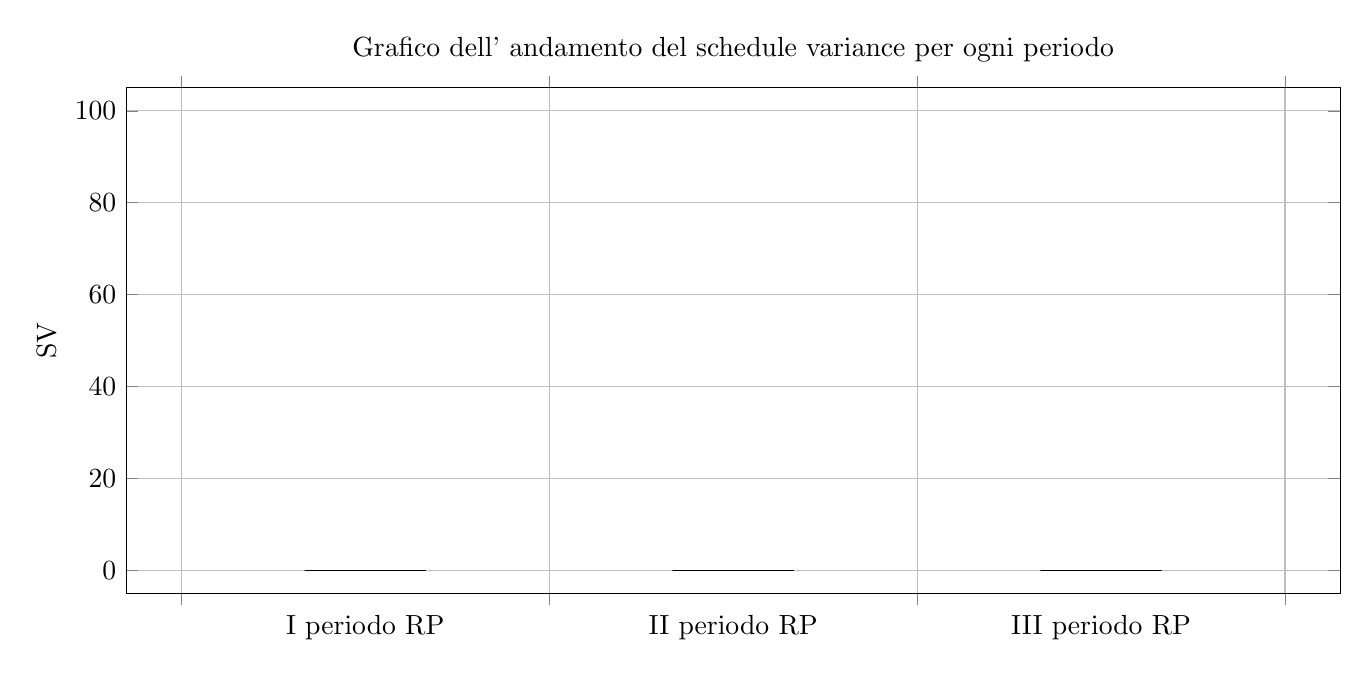
\begin{tikzpicture}

\begin{axis}[
title=Grafico dell' andamento del schedule variance per ogni periodo,
x tick label style={
	/pgf/number format/1000 sep=},
ylabel=SV,
enlargelimits=0.05,
legend style={at={(0.5,-0.4)},
	anchor=north,legend columns=-1},
ybar interval=0.33,
symbolic x coords={I periodo RP, II periodo RP, III periodo RP, tmp},%lasciare tmp come ultima colonna per poter visualizzare tutte le colonne tranne tmp
grid=major,
xtick=data
]
\addplot[fill=blue] coordinates
{(I periodo RP, 0) (II periodo RP, 0) (III periodo RP, 0) (tmp, 100)};

\end{axis}
\end{tikzpicture}

\paragraph{MPC12 - Budget Variance}
\pgfplotsset{width=17cm, height=8cm}
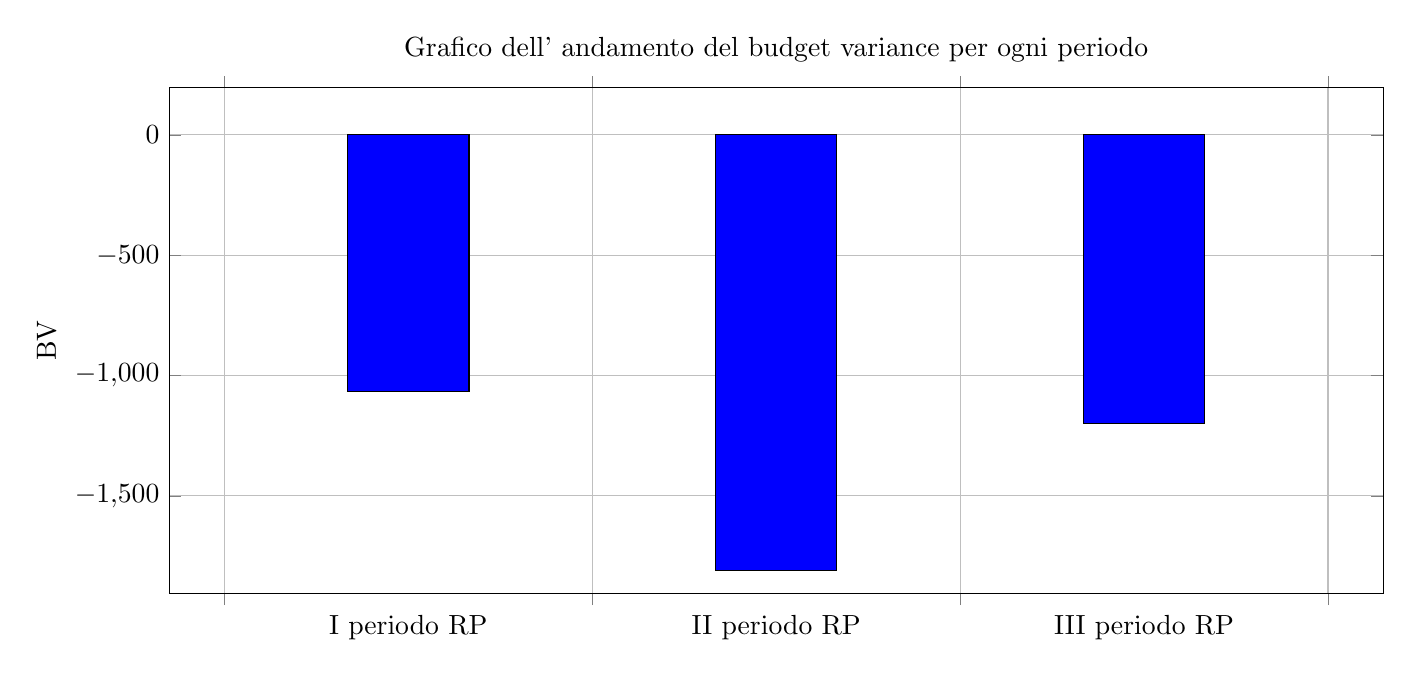
\begin{tikzpicture}

\begin{axis}[
title=Grafico dell' andamento del budget variance per ogni periodo,
x tick label style={
	/pgf/number format/1000 sep=},
ylabel=BV,
enlargelimits=0.05,
legend style={at={(0.5,-0.4)},
	anchor=north,legend columns=-1},
ybar interval=0.33,
symbolic x coords={I periodo RP, II periodo RP, III periodo RP, tmp},%lasciare tmp come ultima colonna per poter visualizzare tutte le colonne tranne tmp
grid=major,
xtick=data
]
\addplot[fill=blue] coordinates
{(I periodo RP, -1065) (II periodo RP, -1809) (III periodo RP, -1200) (tmp, 100)};

\end{axis}
\end{tikzpicture}

\newpage
\paragraph{MPD1 - Attrattività della User Interface (UI)}
\subparagraph*{Legenda}
\begin{itemize}
	\item \textbf{0} = Non valutato;
	\item \textbf{1} = Non Attrattivo;
	\item \textbf{2} = Poco attrattivo;
	\item \textbf{3} = Attrattivo;
	\item \textbf{4} = Molto attrattivo. 
\end{itemize}

\pgfplotsset{width=17cm, height=8cm}
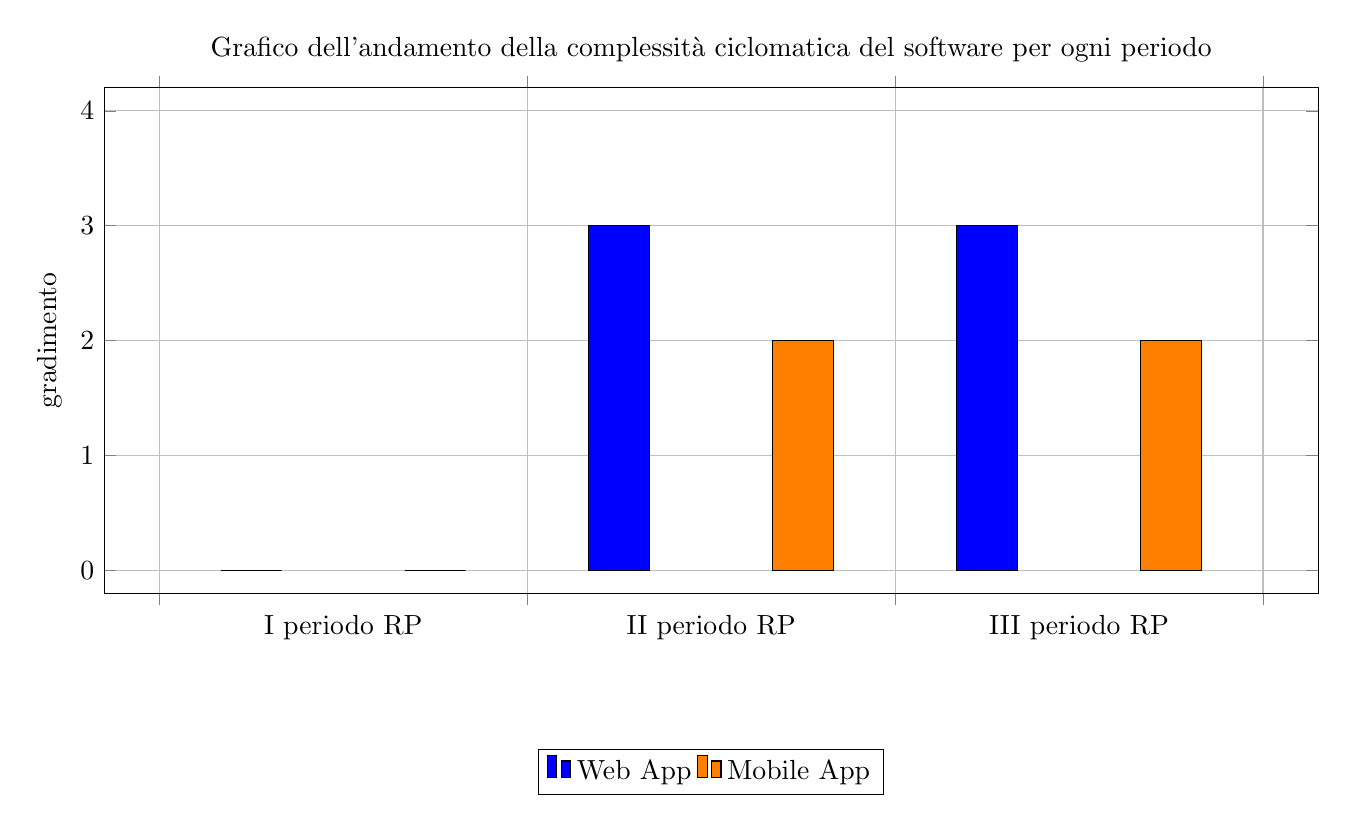
\begin{tikzpicture}

\begin{axis}[
title=Grafico dell'andamento della complessità ciclomatica del software per ogni periodo,
x tick label style={
	/pgf/number format/1000 sep=},
ylabel=gradimento,
enlargelimits=0.05,
legend style={at={(0.5,-0.4)},
	anchor=north,legend columns=-1},
ybar interval=0.33,
symbolic x coords={I periodo RP, II periodo RP, III periodo RP, tmp},%lasciare tmp come ultima colonna per poter visualizzare tutte le colonne tranne tmp
grid=major,
legend style={at={(0.5,-0.4)},
	anchor=south,legend columns=-1},
xtick=data
]
\addplot[fill=blue] coordinates
{(I periodo RP, 0) (II periodo RP, 3) (III periodo RP, 3) (tmp, 4)};
\addplot[fill=orange] coordinates
{(I periodo RP, 0) (II periodo RP, 2) (III periodo RP, 2) (tmp, 4)};

\legend{
	Web App,
	Mobile App
}
\end{axis}
\end{tikzpicture}

\paragraph{MPD2 - Complessità Ciclomatica del Software}
\pgfplotsset{width=17cm, height=8cm}
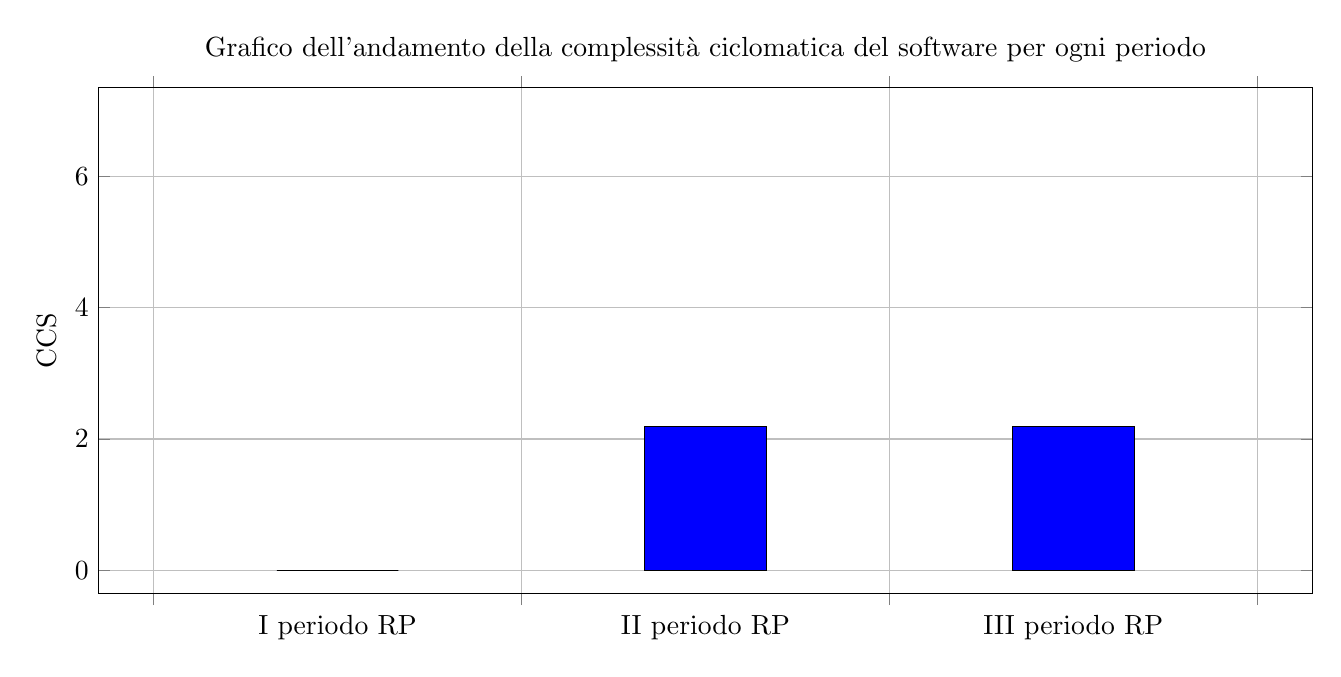
\begin{tikzpicture}

\begin{axis}[
title=Grafico dell'andamento della complessità ciclomatica del software per ogni periodo,
x tick label style={
	/pgf/number format/1000 sep=},
ylabel=CCS,
enlargelimits=0.05,
legend style={at={(0.5,-0.4)},
	anchor=north,legend columns=-1},
ybar interval=0.33,
symbolic x coords={I periodo RP, II periodo RP, III periodo RP, tmp},%lasciare tmp come ultima colonna per poter visualizzare tutte le colonne tranne tmp
grid=major,
xtick=data
]
\addplot[fill=blue] coordinates
{(I periodo RP, 0) (II periodo RP, 2.19) (III periodo RP, 2.19) (tmp, 7)};

\end{axis}
\end{tikzpicture}

\paragraph{MPD3 - Unità Documentate}
\pgfplotsset{width=17cm, height=8cm}
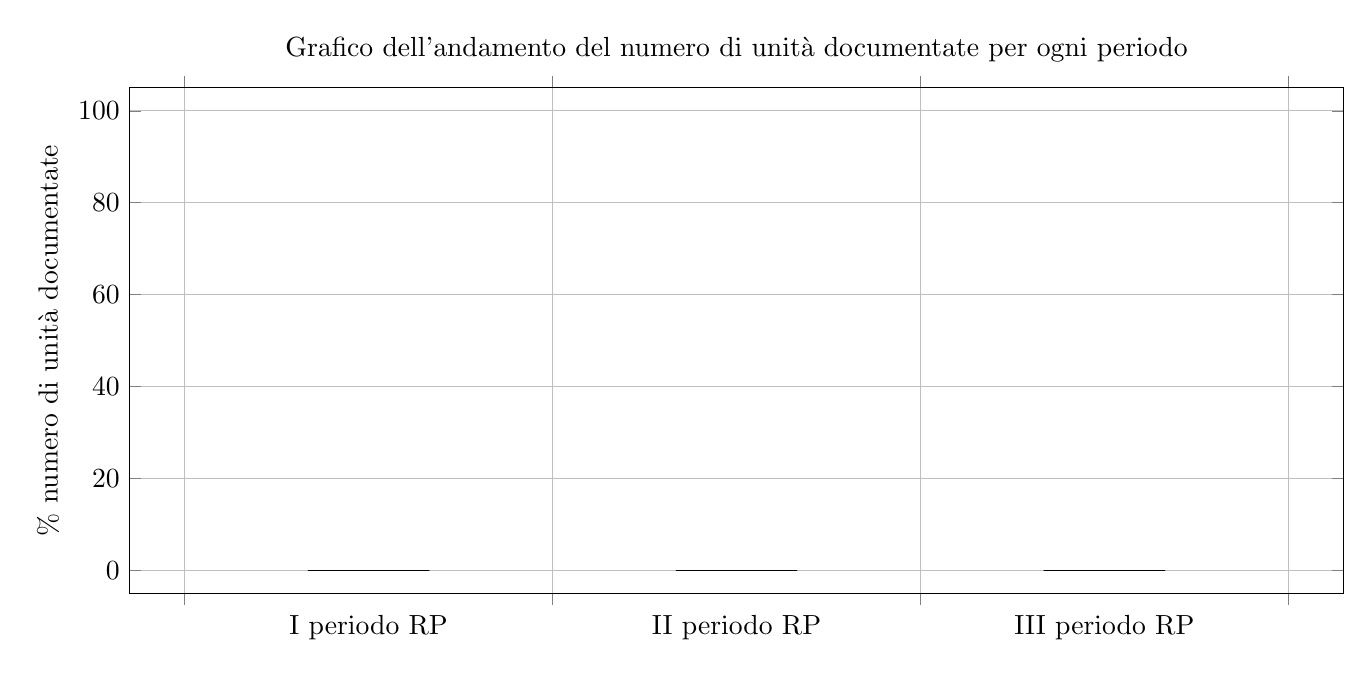
\begin{tikzpicture}

\begin{axis}[
title=Grafico dell'andamento del numero di unità documentate per ogni periodo,
x tick label style={
	/pgf/number format/1000 sep=},
ylabel=\% numero di unità documentate,
enlargelimits=0.05,
legend style={at={(0.5,-0.4)},
	anchor=north,legend columns=-1},
ybar interval=0.33,
symbolic x coords={I periodo RP, II periodo RP, III periodo RP, tmp},%lasciare tmp come ultima colonna per poter visualizzare tutte le colonne tranne tmp
grid=major,
xtick=data
]
\addplot[fill=blue] coordinates
{(I periodo RP, 0) (II periodo RP, 0) (III periodo RP, 0) (tmp, 100)};

\end{axis}
\end{tikzpicture}

\paragraph{MPD4 - Presenza di Code Smell}
\pgfplotsset{width=17cm, height=8cm}
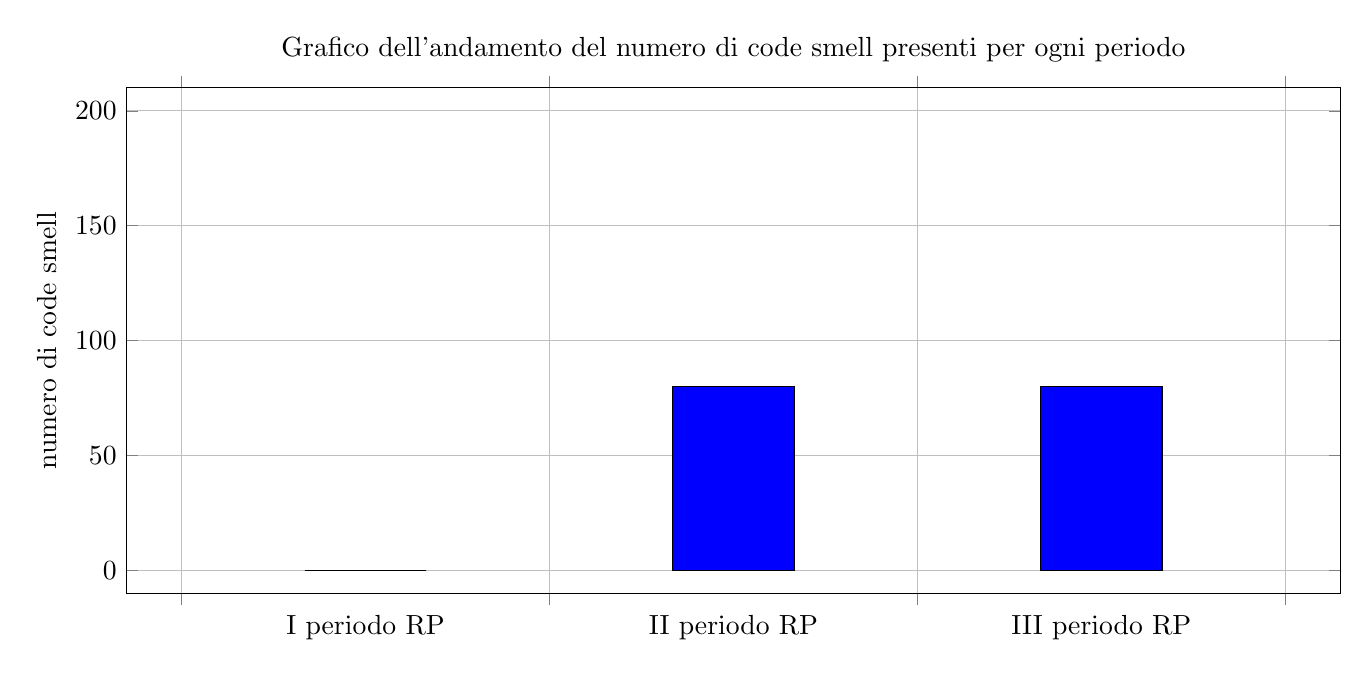
\begin{tikzpicture}

\begin{axis}[
title=Grafico dell'andamento del numero di code smell presenti per ogni periodo,
x tick label style={
	/pgf/number format/1000 sep=},
ylabel=numero di code smell,
enlargelimits=0.05,
legend style={at={(0.5,-0.4)},
	anchor=north,legend columns=-1},
ybar interval=0.33,
symbolic x coords={I periodo RP, II periodo RP, III periodo RP, tmp},%lasciare tmp come ultima colonna per poter visualizzare tutte le colonne tranne tmp
grid=major,
xtick=data
]
\addplot[fill=blue] coordinates
{(I periodo RP, 0) (II periodo RP, 80) (III periodo RP, 80) (tmp, 200)};

\end{axis}
\end{tikzpicture}

\paragraph{MPD5 - Presenza di Vulnerabilità}
\pgfplotsset{width=17cm, height=8cm}
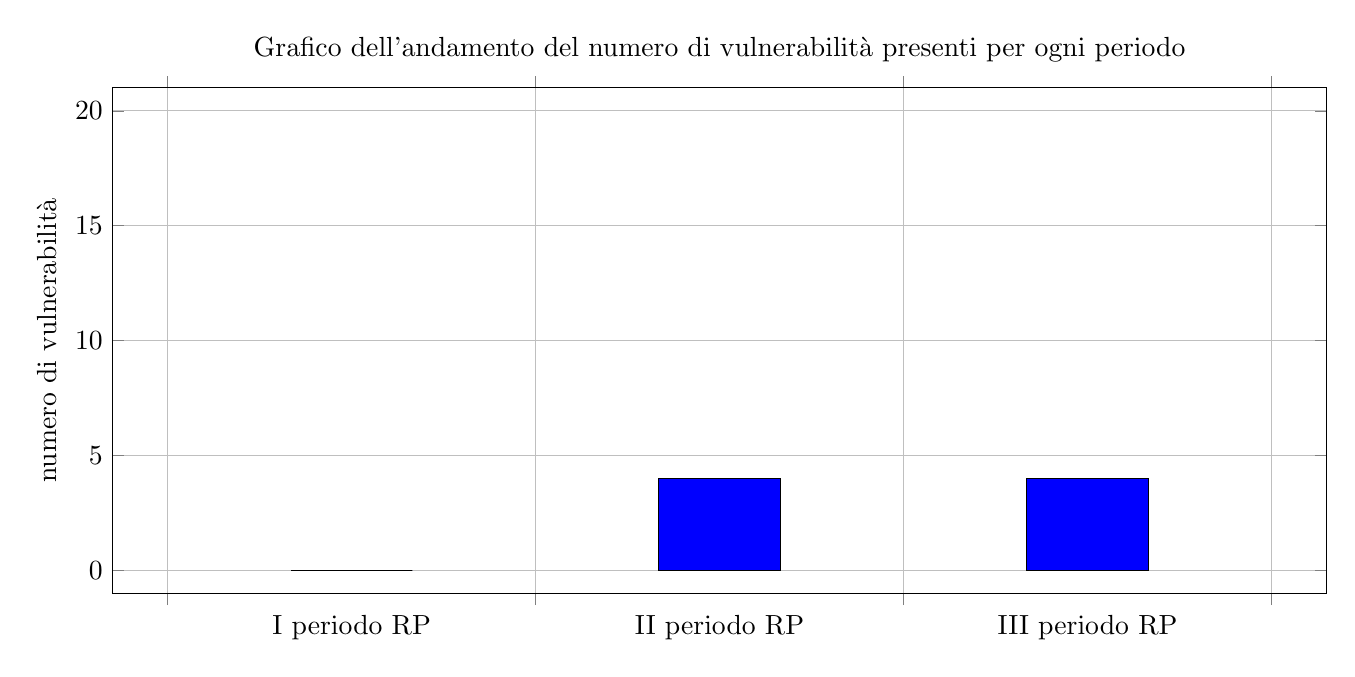
\begin{tikzpicture}

\begin{axis}[
title=Grafico dell'andamento del numero di vulnerabilità presenti per ogni periodo,
x tick label style={
	/pgf/number format/1000 sep=},
ylabel=numero di vulnerabilità,
enlargelimits=0.05,
legend style={at={(0.5,-0.4)},
	anchor=north,legend columns=-1},
ybar interval=0.33,
symbolic x coords={I periodo RP, II periodo RP, III periodo RP, tmp},%lasciare tmp come ultima colonna per poter visualizzare tutte le colonne tranne tmp
grid=major,
xtick=data
]
\addplot[fill=blue] coordinates
{(I periodo RP, 0) (II periodo RP, 4) (III periodo RP, 4) (tmp, 20)};

\end{axis}
\end{tikzpicture}

\paragraph{MPD6 - Presenza di Bug}
\pgfplotsset{width=17cm, height=8cm}
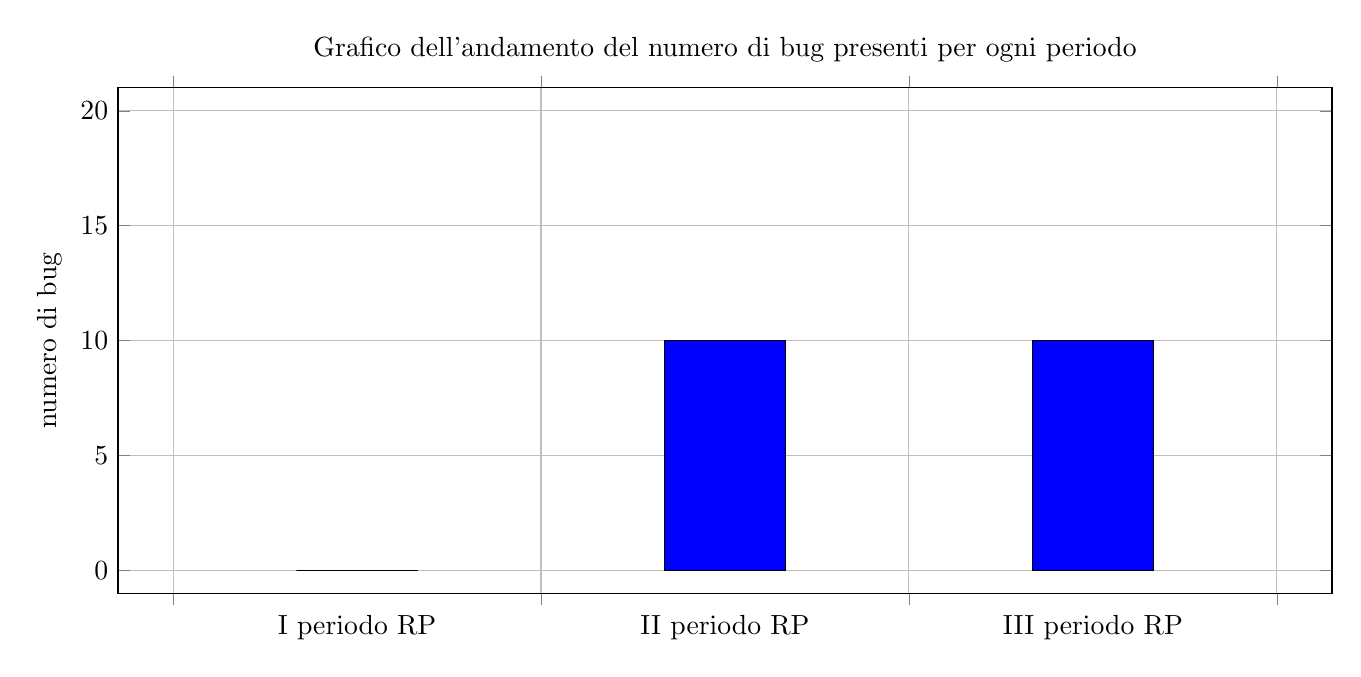
\begin{tikzpicture}

\begin{axis}[
title=Grafico dell'andamento del numero di bug presenti per ogni periodo,
x tick label style={
	/pgf/number format/1000 sep=},
ylabel=numero di bug,
enlargelimits=0.05,
legend style={at={(0.5,-0.4)},
	anchor=north,legend columns=-1},
ybar interval=0.33,
symbolic x coords={I periodo RP, II periodo RP, III periodo RP, tmp},%lasciare tmp come ultima colonna per poter visualizzare tutte le colonne tranne tmp
grid=major,
xtick=data
]
\addplot[fill=blue] coordinates
{(I periodo RP, 0) (II periodo RP, 10) (III periodo RP, 10) (tmp, 20)};

\end{axis}
\end{tikzpicture}

\paragraph{MPD8 - Profondità Strutturale dell'Interfaccia}
\pgfplotsset{width=17cm, height=8cm}
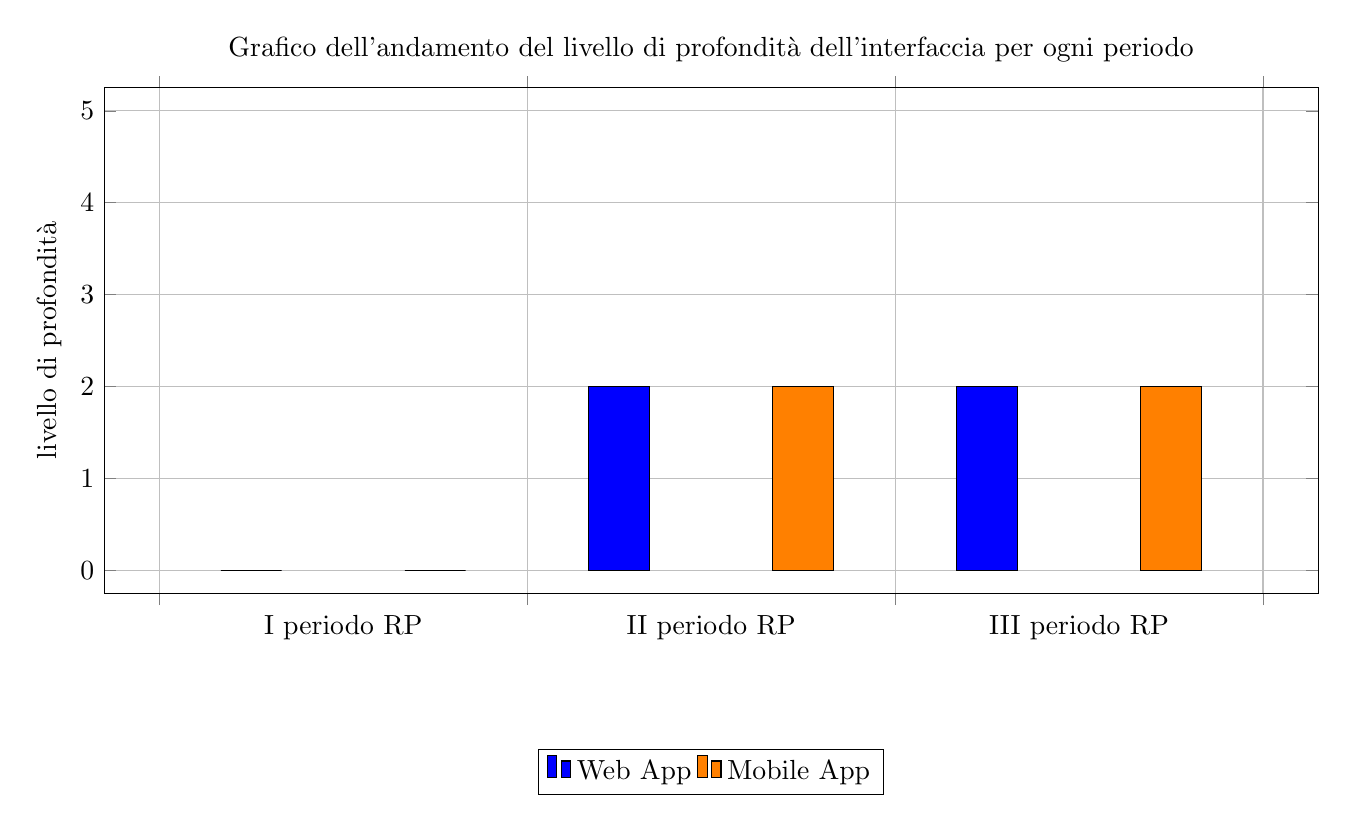
\begin{tikzpicture}

\begin{axis}[
title=Grafico dell'andamento del livello di profondità dell'interfaccia per ogni periodo,
x tick label style={
	/pgf/number format/1000 sep=},
ylabel=livello di profondità,
enlargelimits=0.05,
legend style={at={(0.5,-0.4)},
	anchor=north,legend columns=-1},
ybar interval=0.33,
symbolic x coords={I periodo RP, II periodo RP, III periodo RP, tmp},%lasciare tmp come ultima colonna per poter visualizzare tutte le colonne tranne tmp
grid=major,
legend style={at={(0.5,-0.4)},
	anchor=south,legend columns=-1},
xtick=data
]
\addplot[fill=blue] coordinates
{(I periodo RP, 0) (II periodo RP, 2) (III periodo RP, 2) (tmp, 5)};

\addplot[fill=orange] coordinates
{(I periodo RP, 0) (II periodo RP, 2) (III periodo RP, 2) (tmp, 5)};

\legend{
	Web App,
	Mobile App
}

\end{axis}
\end{tikzpicture}

\subsubsection{Analisi esiti ottenuti}
Le misurazioni sono state fatte nei tre periodi indicati nel documento \PdP{} e disponibili fino al momento della consegna.
Nel primo periodo sono stati corretti i documenti, nel secondo il gruppo \Gruppo{} si è impegnato nella realizzazione del \glo{Proof of Concept}, infine nel terzo si sono aggiornati i vari documenti.
Nel quarto periodo, dal momento della consegna fino alla RP si procederà secondo la pianificazione definita nel \PdP{}.
Nelle metriche applicate al \glo{Proof of Concept} il primo periodo non sarà valorizzato, mentre il secondo e il terzo avranno valori uguali. Questo perché nel primo non esisteva il \glo{Proof of Concept} mentre nel terzo periodo non lo si è modificato.\\ 
Nella realizzazione del \glo{Proof of Concept} il gruppo \Gruppo{} ha scelto di non concentrarsi molto sulla qualità del prodotto ma di concentrarsi nel realizzare un prodotto con lo scopo di misurare la nostra capacità di "addomesticare" le tecnologie scelte per realizzare il prodotto richiesto.
Si hanno quindi alcune metriche applicate al \glo{PoC} che ottengono buoni risultati, mentre in altre si ottengono risultati non soddisfacenti.
Purtroppo al fine di avere un \glo{PoC} funzionante nel tempo prestabilito non si è potuto implementare dei test perciò le metriche \textbf{MPC7} e \textbf{MPD7} risultano essere non applicabili ora.\\
Buoni risultati si sono ottenuti nelle metriche \textbf{MPC8}, \textbf{MPC9}, \textbf{MPC10}, \textbf{MPC11} e \textbf{MPD12}, le quali mostrano che il gruppo \Gruppo{} è in linea con quanto aveva preventivato nel documento \PdP{}.